\lab{Modelling the spread of an epidemic: SIR models}{Modelling the spread of an epidemic: SIR models}
\label{lab:SIRModels}
\labdependencies{IVPBVPIntro}

\section*{Numerical Solvers}
We often rely on numerical solvers to numerically integrate ordinary differential equations (ODEs), especially for complicated and high-dimensional systems with no symbolic solution.
In this lab we will be using \li{solve_ivp}, which is a part of \li{scipy.integrate}, to solve ODE systems related to epidemic models.
You can read the documentation for \li{solve_ivp} at \url{https://docs.scipy.org/doc/scipy/reference/generated/scipy.integrate.solve_ivp.html}.

As we discussed in the previous lab, Intro to IVPs and BVPs, \li{solve_ivp} takes the ODE as a function, a tuple containing the start and end time, and an array with the initial conditions as arguments, and returns a bunch object containing the solution and other information.
We can solve the following ODE system with the following code:
\begin{equation}\label{ex:ivp-example}
    \begin{aligned}
    \begin{bmatrix} y_1(t) \\ y_2(t)\end{bmatrix}'
    &= \begin{bmatrix} y_2(t) \\ \sin(t) - 5y_2(t) - y_1(t) \end{bmatrix} \\
    y_1(0) = &0, \quad y_2(0)=1, \quad t\in[0,3\pi]
    \end{aligned}
\end{equation}
\begin{lstlisting}
import numpy as np
from scipy.integrate import solve_ivp

# define the ode system as given in the problem
def ode(t,y):
    return np.array([y[1], np.sin(t) - 5*y[1] - y[0]])

# define the t0 and tf parameters
t0 = 0
tf = 3*np.pi

# define the initial conditions
y0 = np.array([0,1])

# solve the system
sol = solve_ivp(ode, (t0,tf), y0, t_eval=np.linspace(t0, tf, 150))

# Plot the system
import matplotlib.pyplot as plt

# plot y_1 against y_2
plt.plot(sol.y[0],sol.y[1])
plt.xlabel('$y_1$')
plt.ylabel('$y_2$')
plt.show()
\end{lstlisting}

\begin{figure}[ht]
    \centering
    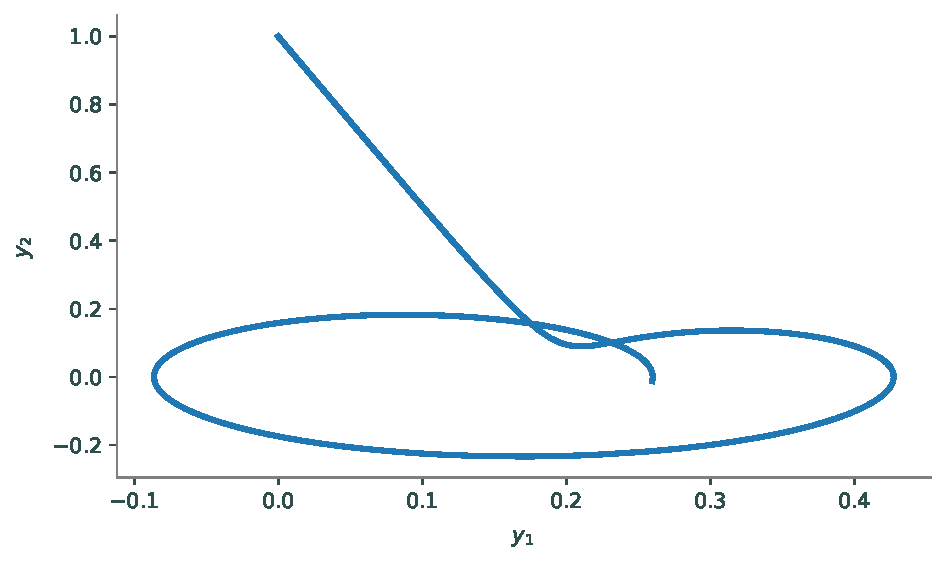
\includegraphics[width=\textwidth]{figures/ivpexample1.pdf}
    \caption{Solution to the example given by Equation (\ref{ex:ivp-example})}
    \label{fig:ivp-example}
\end{figure}



\section*{The SIR Model}
The SIR model describes the spread of an epidemic through a large population.
It does this by describing the movement of the population through three phases of the disease: those individuals who are \emph{susceptible}, those who are \emph{infectious}, and those who have been \emph{removed} from the disease.
Those individuals in the removed class have either died, or have recovered from the disease and are now immune to it.
If the outbreak occurs over a short period of time, we may reasonably assume that the total population is fixed, so that $S'(t) + I'(t) + R'(t) = 0$.
We may also assume that $S(t) + I(t) + R(t) = 1$, so that $S(t)$ represents the \textit{fraction} of the population that is susceptible, etc.

Individuals may move from one class to another as described by the flow
\[S \to I \to R.\]
Let us consider the transition rate between $S$ and $I $.
Let $\beta$ represent the average number of contacts made per unit time period (one day perhaps) that could spread the disease.
The proportion of these contacts that are with a susceptible individual is $S(t)$.
Thus, one infectious individual will on average infect $\beta S(t)$ others per day.
Let $N$ represent the total population size.
Then we obtain the differential equation
\[\frac{d}{dt}(S(t) N) = -\beta S(t) (I(t) N)\]

Now consider the transition rate between $I$ and $R$.
We assume that there is a fixed proportion $\gamma$ of the infectious group who will recover on a given day, so that
\[\frac{d}{dt}R(t) = \gamma I(t).\]
Note that $\gamma$ is the reciprocal of the average length of time spent in the infectious phase.

Since the derivatives sum to $0$, we have $I'(t) = - S'(t) - R'(t)$, so the  differential equations are given by
\begin{align}
\frac{dS}{dt} &=-\beta IS ,\\
\frac{dI}{dt} &= \beta I S-\gamma I,\\
\frac{dR}{dt} &=\gamma I.
\end{align}

\begin{problem}\label{sir_prob1}
Suppose that, in a city of approximately three million, five people have recently entered the city carrying a certain disease.
Each infected individual has one contact each day that could spread the disease, and an average of three days is spent in the infectious state.

Find the solution of the corresponding SIR equations using \li{solve_ivp} over a time period of fifty days, and plot your results.
Compare your plot to Figure \ref{sir_prob1}.
Use the percentages of each state, not the actual number of people in the state.

At the peak of the infection, how many in the city will still be able to work (assume for simplicity that those who are in the infectious state either cannot go to work or are unproductive, etc.)?

Hint: Use the \li{t_eval} argument of \li{solve_ivp} to specify the points in time that you want the solution's value at.
This parameter accepts a linspace of time values.
Specify enough points that your graph is smooth.
\end{problem}

\begin{figure}[H]
\centering
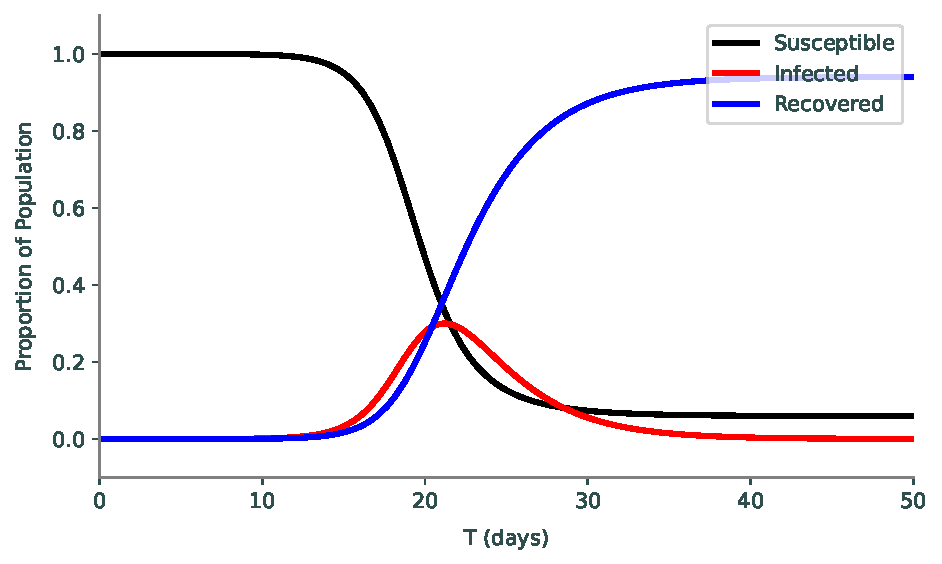
\includegraphics[width=\textwidth]{figures/SIR1.pdf}
\caption{Solution to Problem \ref{sir_prob1}}
\label{sir1}
\end{figure}

SIR is an effective model for epidemic spread under certain assumptions.
For example, we assume that the network is what's called ``fully mixed.''
This implies that no group of members of a network are more likely to encounter each other than any other group.
Because of this assumption, we should not use SIR to model networks we know to be poorly mixed.
In fact, we should be clear in stating that almost no network is truly fully mixed; however this model is still effective for networks that are reasonably well mixed.
In the next problem we will be using SIR to model data from the recent COVID-19 outbreak.
To adhere to the ``reasonably well mixed'' criteria, we will be using only data from one county at a time.

\begin{problem}
\label{prob:sir:nyc}
On March 11, 2020, New York City had 52 confirmed cases of COVID-19.
On that day, New York started its lock-down measures.
Using the following information, model what the spread of the virus could have been, using \li{solve_ivp()}, if New York did not implement any measures to curb the spread of the virus over the next 150 days:

\begin{itemize}
    \item There are approximately 8.399 million people in New York City.
    \item The average case of COVID-19 lasts for 10 days.
    \item Each infected person spreads the virus to $2.5$ people on average over the whole time that they are sick.
\end{itemize}

Plot your results for each day and compare to Figure \ref{fig:sir:nyc-sol}.
Also answer the following questions:
\begin{enumerate}
\item At the projected peak, how many concurrent active cases are there?
\item Assuming that about 5\% of COVID-19 cases require hospitalization, and using the fact that there are about 58,000 hospital beds in NYC, how many beds over capacity will the hospitals in NYC be at the projected peak?
\end{enumerate}

Hint: Recall that $\beta$ is the average number of contacts an infected person makes per day that could spread the disease, and $\gamma$ is the reciprocal of the average length of time spent in the infectious phase.
\end{problem}


\begin{figure}[h]
\centering
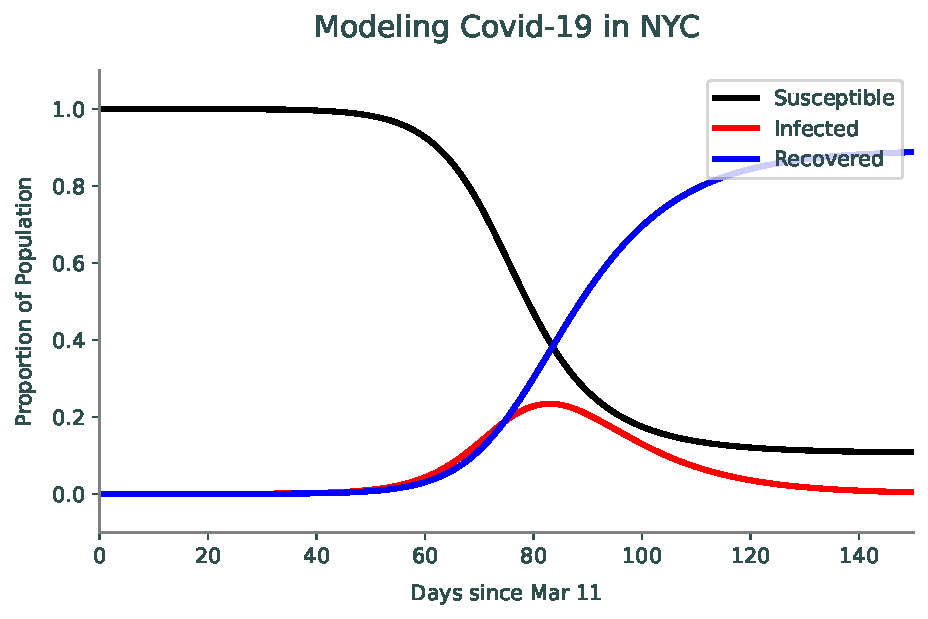
\includegraphics[width=\textwidth]{figures/SIR2.pdf}
\caption{Solution to Problem \ref{prob:sir:nyc}.}
\label{fig:sir:nyc-sol}
\end{figure}


\section*{Variations on the SIR Model}

The SIS model is a common variation of the SIR model.
SIS Models describe diseases where individuals who have recovered from the disease do not gain any lasting immunity.
There are only two compartments in this model: those who are \emph{susceptible}, and those who are \emph{infectious}.
Here, $f$ is the rate of becoming susceptible again.

The basic equations are given by
\begin{align*}
\frac{dS}{dt} &=-\beta I S + fI ,\\
\frac{dI}{dt} &= \beta I S - fI
\end{align*}

Another alteration we can make to the SIR model is to add a birth and death rate.
In the equations below we are assuming that the natural death rate together with the death rate caused by the disease is equal to the birth rate. This model is given by
\begin{align*}
\frac{dS}{dt} &=\mu(1 -S) - \beta I S,\\
\frac{dI}{dt} &= \beta I S - (\gamma + \mu)I, \\
\frac{dR}{dt} &= \gamma I - \mu R
\end{align*}
where $\mu$ represents the death rate and equal birth rate, noting that any new person born is born into the susceptible population.

If we combine the last two variations we made on the SIR model we come to this formulation, which is an SIRS model.
This SIRS model allows the transfer of individuals from the recovered/removed class to the susceptible class and includes modeling of the birth and death rates.
\begin{align}
\frac{dS}{dt} &= fR + \mu(1 -S) - \beta I S,\\
\frac{dI}{dt} &= \beta I S - (\gamma + \mu)I, \\
\frac{dR}{dt} &= -fR + \gamma I - \mu R.
\end{align}

\begin{problem}
\label{prob:sir:flu}
There are 7 billion people in the world.
Influenza, or the flu, is one of those viruses that everyone can be susceptible to, even after recovering.
The flu virus is able to change in order to evade our immune system, and we become susceptible once more, although technically it is now a different strain.

Suppose the virus originates with 1000 people in Texas after Hurricane Harvey flooded Houston, and stagnant water allowed the virus to proliferate.
%According to WebMD, once you get the virus, adults are contagious up to a week and kids up to 2 weeks.
Suppose the average person is contagious for 10 days before recovering.
Also suppose that on average someone makes one contact every two days that could spread the flu.
Since we can catch a new strain of the flu, suppose that a recovered individual becomes susceptible again with rate $f=1/50$.
The flu is also known to be deadly, killing hundreds of thousands every year on top of the normal death rate.
To assure a steady population, let the birth rate balance out the death rate, and let $\mu=0.0001$.

Using the SIRS model above, plot the proportion of population that is Susceptible, Infected, and Recovered over a one-year span (365 days).
Compare your plot to Figure \ref{fig:sir:flu-sol}.
\end{problem}

\begin{figure}[H]
\centering
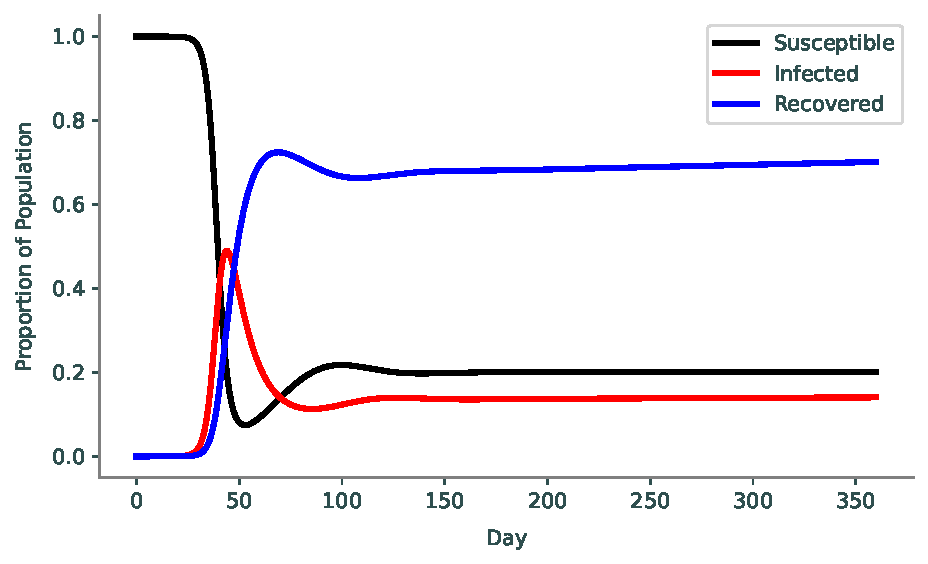
\includegraphics[width=\textwidth]{figures/problem3.pdf}
\caption{Solution to Problem \ref{prob:sir:flu}.}
\label{fig:sir:flu-sol}
\end{figure}


\subsection*{Modeling COVID-19 with Social Distancing}

Social distancing upsets the main assumption that is made when trying to model epidemic spread using SIR models.
During the periods of lockdown instituted by governments, the interaction networks between people in a city or county were disrupted to the point that standard SIR models were no longer effective at modeling the spread of COVID-19.
A \href{https://arxiv.org/pdf/2005.06933.pdf}{paper released in May of 2020} presented some alternative models for COVID-19 that have some success in modeling its spread during periods of social distancing.

This model claims that the growth of $I(t)$ is polynomial with exponential decay (PGED),
%So we get the following form
%\begin{align*}
%    I(t) \approx Bt^\alpha e^{-t/T_G},
%\end{align*}
which results in the following SIR type model:
\begin{align}
    \frac{dS}{dt} &= -\frac{\alpha}{t}I, \label{eq:sir:covid-model-1}\\
    \frac{dI}{dt} &= \left(\frac{\alpha}{t} - \frac{1}{T_G}\right)I, \label{eq:sir:covid-model-2}\\
    \frac{dR}{dt} &= \frac{1}{T_G}I. \label{eq:sir:covid-model-3}
\end{align}
The values $\alpha$ and $T_G$ are the model parameters.
The product $\alpha T_G$ can be interpreted as the time of epidemic peak.

\subsubsection*{Fitting Models}

Model fitting can be a frustrating task if we only use our intuition and guess and check.
Thankfully, SciPy's \li{optimize} library has tools we can use to make these problems a lot easier.
We will use \li{scipy.optimize.minimize} to find the parameters that minimize the error between the model and the actual data.

Suppose we have some data that we believe to follow a cubic trend with the following model
\begin{align*}
    \alpha x^3 + \beta (x^2 + 2x) + \delta.
\end{align*}
We will create a function that calculates the error of the model against the data, and pass it into \li{scipy.optimize.minimize}.
This function will accept an array containing all of the parameters, and return a floating-point value.
The function \li{scipy.optimize.minimize} will then return an \li{OptimizeResult} object, which contains the optimal parameters.

\begin{lstlisting}
# import the minimizer function
from scipy.optimize import minimize

# Load the data and get the x and y values
data = np.load('to_fit.npy')
xs = data[:,0]
ys = data[:,1]

# define the function we want to minimize
def calculate_error(params):
    # Unpack the parameters
    a,b,d = params

    # Get the model output based on the parameters
    model_prediction = a*xs**3 + b*(xs**2 + 2*xs) + d

    # Find the difference between out and the data
    diff = model_prediction - ys

    # Calculate the error
    return np.linalg.norm(diff)

# Make a guess for the parameters
p0 = (1,1,1)

# Find the best parameters for this model
result = minimize(fun,p0)

# Get the minimizer
print(result.x)
\end{lstlisting}


\begin{problem}\label{sir_nyc-model}
    The file \li{new_york_cases.npy} contains daily case counts for COVID-19 beginning on March 11, 2020.
    These counts are the total number of people who have been sick at any time up to that point; that is, the sum of the number of people currently infected and the number of people who have recovered, corresponding to $I(t)+R(t)$.
    
    Convert the counts from the file to proportions of New York's population (recall that the total population is 8.399 million people).
    Fit the PGED model to the COVID-19 data by using \li{scipy.optimize.minimize} to find values of $\alpha$ and $T_G$ that minimize the difference between the observed proportions and the model's prediction for $I(t)+R(t)$.
    Unlike the example above, in this problem our model is the system of ODEs \eqref{eq:sir:covid-model-1}, \eqref{eq:sir:covid-model-2}, and \eqref{eq:sir:covid-model-3} rather than an explicit formula.
    So, to find \li{model_output} in the function you pass into \li{scipy.optimize.minimize}, you will need to use \li{solve_ivp} to solve the system of ODEs every time the function is called.
    
    Plot the actual data alongside the values of $I(t)+R(t)$ predicted by your model.
    Print the values of $\alpha$ and $T_G$ you found.

    Hint: Set $t_0=1$; the PEGD model requires dividing by $t$, so we must have $t\ne0$.
    To pass the values of $\alpha$ and $T_G$ into your ODE function, you can use the argument \li{args=(alpha, T_G)} inside \li{solve_ivp}.
    Use the \li{t_eval} argument to get the ODE solution values at the correct times.
\end{problem}

\begin{figure}[H]
    \centering
    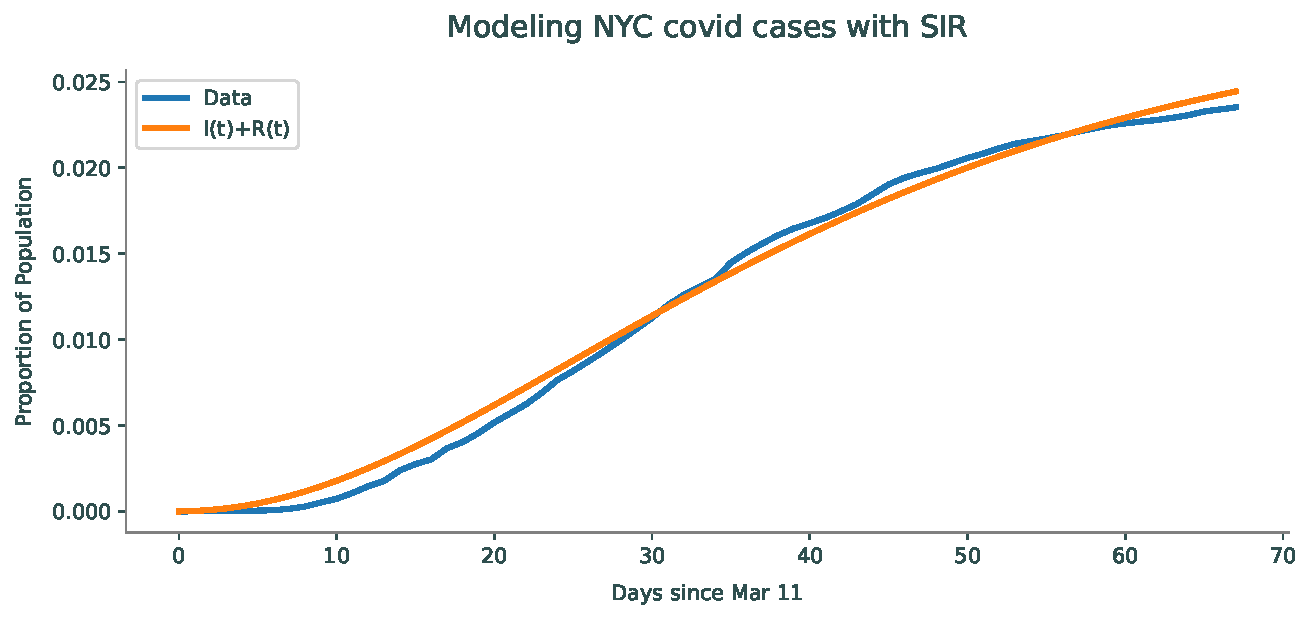
\includegraphics[width=\textwidth]{figures/PGED-model.pdf}
    \caption{Solution to Problem \ref{sir_nyc-model}}
    \label{nyc_ex}
\end{figure}



\section*{Boundary Value Problems}

The next exercise uses a variation of the SIR model called an SEIR model to describe the spread of measles.\footnote{Numerical Solution of Boundary Value Problems for Ordinary Differential Equations, by Aescher, Mattheij, and Russell}
This new model adds another compartment, called the \emph{exposed} or \emph{latency} phase.
It assumes that the rate at which measles is contracted depends on the season, i.e. the rate is periodic.
That allows us to formulate the yearly occurrence rate for measles as a boundary value problem.
The boundary value problem looks like
\begin{equation}\label{SEIR_BVP}
\left[\begin{array}{c}S \\ E \\ I\end{array}\right]' = \left[\begin{array}{c}\mu - \beta(t) S I \\\beta(t) SI - E/\lambda \\E/\lambda - I/\eta\end{array}\right],
\end{equation}
\begin{equation}\label{SEIR_BC}
    \begin{aligned}
        S(0) &= S(1),\\
        E(0) &= E(1),\\
        I(0) &= I(1)
    \end{aligned}
\end{equation}

The parameters $\mu$ and $\lambda$ represent the birth rate of the population and the latency period of measles, respectively.
The parameter $\eta$ represents the length of the infectious period before an individual moves from the infectious class to the recovered class.
After recovery an individual remains immune, which is why $R(t)$ is not included in the system.
The set up of this problem is not normal since we are excluding $R(t)$, but it results in a nice graph.

To solve this problem we will use the BVP solver available in SciPy.
As a refresher, the code below demonstrates how to use \li{solve_bvp} to solve the BVP
\begin{align}\label{simple_bvp}
	\epsilon y'' + yy' - y &= 0, \quad y(-1) = 1, \quad y(1) = -1/3, \quad \epsilon=0.1.
\end{align}
See Figure \ref{bvp_ex} for the solution.

The BVP solver requires a callable function for the boundary conditions.
This function needs to compute the difference between the value of the current guess at the boundary conditions and the desired boundary conditions.
In this case, we have one boundary condition on either side.
These constraints will evaluate to 0 precisely when the boundary condition is satisfied.

\begin{lstlisting}
import numpy as np
from scipy.integrate import solve_bvp
import matplotlib.pyplot as plt

epsilon, lbc, rbc = 0.1, 1, -1/3

# The ode function takes the independent variable first
# It has return shape (n,)
def ode(x , y):
    return np.array([
        y[1] , 
        (1/epsilon) * (y[0] - y[0] * y[1])
    ])

# The return shape of bcs() is (n,)
def bcs(ya, yb):
    # The return values will be 0s when the boundary conditions are met exactly
    return np.array([
    	ya[0] - lbc, # One boundary condition on the left
         yb[0] - rbc, # One boundary condition on the right
    ])

# The independent variable has size (m,) and goes from a to b
t = np.linspace(-1, 1, 200)
# The initial guess for y must have shape (n,m)
y_guess = np.array([-1/3, -4/3]).reshape((-1,1))*np.ones((2, len(t)))

# Solve the BVP
solution = solve_bvp(ode, bcs, t, y_guess)
# The returned object has multiple objects. We will use sol, which is a
#     callable function of the solution. We are interested in only y, 
#     which is the first row.
y_plot = solution.sol(t)[0]

# You can also instead use sol.x and sol.y. Note that these will not 
#     be the same lengths as your initial guesses.

plt.plot(t, y_plot)
plt.xlabel('t')
plt.ylabel('y')
plt.show()
\end{lstlisting}
\begin{figure}[H]
    \centering
    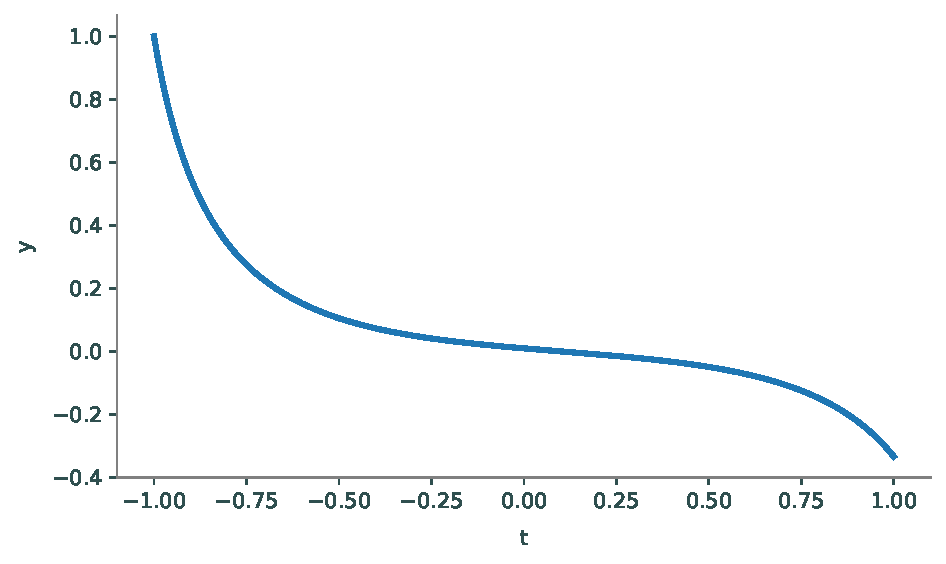
\includegraphics[width=\textwidth]{figures/bvp_example.pdf}
    \caption{Solution to the example given by Equation \eqref{simple_bvp}}
    \label{bvp_ex}
\end{figure}

\begin{problem}
In this problem we will solve the BVP given by equations \eqref{SEIR_BVP} and \eqref{SEIR_BC}.

Let the periodic function for our measles case be $\beta(t) = \beta_0(1 + \beta_1 \cos{2\pi t})$.
Use parameters $\beta_1 = 1,$ $\beta_0 = 1575,$ $\eta = 0.01,$ $\lambda = 0.0279,$ and $\mu = 0.02.$
With these parameter values, time is measured in years, so run the solution over the interval $\left[0, 1\right]$ to show a one-year cycle.
The boundary conditions in \eqref{SEIR_BC} are just saying that the year will begin and end in the same state.

Create functions for the ODE and for the boundary conditions.
Solve the BVP with the given parameters over a period of one year, and plot the values of $S$, $E$, and $I$.
Compare your results with Figure \ref{fig:sir4}.

%When you code your boundary conditions, remember that \li{solve_bvp} changes the initial conditions to force all the entries in the return of \li{bcs()} to be zero.
Hint: Use the initial conditions from Figure \ref{fig:sir4} as your initial guess. 
Remember that the initial infected proportion is small, not 0.

\label{prob:sir_measles}
\end{problem}

\begin{figure}[H]
    \centering
    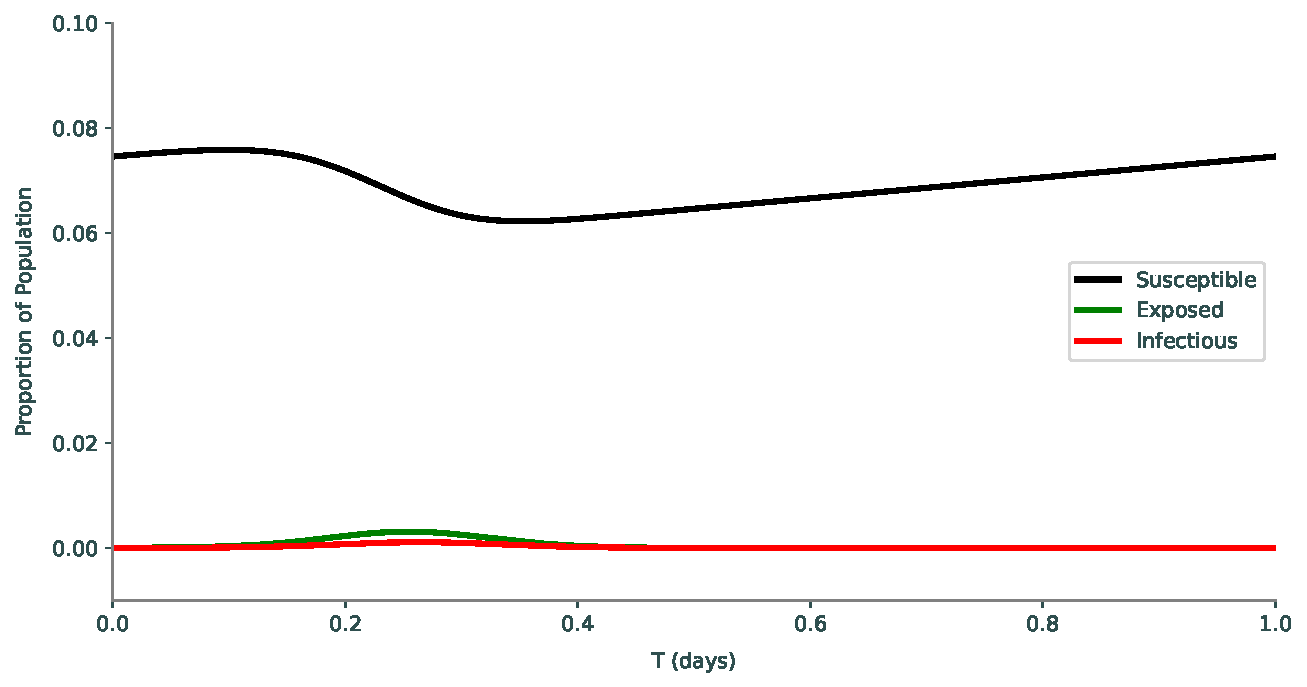
\includegraphics[width=\textwidth]{figures/measles.pdf}
    \caption{Solution to Problem \ref{prob:sir_measles}}
    \label{fig:sir4}
\end{figure}
